\documentclass[fleqn, 11pt]{article}
\usepackage{float}
\usepackage{graphicx}
\usepackage{caption}
\usepackage{subcaption}
\usepackage{enumitem}
\usepackage{booktabs}
\usepackage[portuges]{babel}
\usepackage[utf8x]{inputenc}
\usepackage{comment}
\usepackage{fullpage}
\usepackage{xcolor}
\usepackage{amsmath,amsfonts,amssymb,amsthm, bm}
\usepackage{csvsimple}
\usepackage{amsmath}
\usepackage{listings}
\usepackage{color}
\usepackage{tikz}
\usetikzlibrary{positioning,decorations.pathreplacing}
\usepackage{hyperref}
\setcounter{secnumdepth}{0}
\usepackage{etoolbox}
\usepackage{longtable}

\makeatletter
\patchcmd\l@section{%
  \nobreak\hfil\nobreak
}{%
  \nobreak
  \leaders\hbox{%
    $\m@th \mkern \@dotsep mu\hbox{.}\mkern \@dotsep mu$%
  }%
  \hfill
  \nobreak
}{}{\errmessage{\noexpand\l@section could not be patched}}
\makeatother


\definecolor{mygreen}{RGB}{28,172,0}
\definecolor{mylilas}{RGB}{170,55,241}
\renewcommand{\min}{\expandafter\,\operatorname*{min}}

% Default fixed font does not support bold face
\DeclareFixedFont{\ttb}{T1}{txtt}{bx}{n}{12} % for bold
\DeclareFixedFont{\ttm}{T1}{txtt}{m}{n}{12}  % for normal

% Custom colors
\usepackage{color}
\definecolor{deepblue}{rgb}{0,0,0.5}
\definecolor{deepred}{rgb}{0.6,0,0}
\definecolor{deepgreen}{rgb}{0,0.5,0}

\usepackage{listings}

% Python style for highlighting
\newcommand\pythonstyle{\lstset{
language=Python,
basicstyle=\ttm,
otherkeywords={self},             % Add keywords here
keywordstyle=\ttb\color{deepblue},
emph={MyClass,__init__},          % Custom highlighting
emphstyle=\ttb\color{deepred},    % Custom highlighting style
stringstyle=\color{deepgreen},
frame=tb,                         % Any extra options here
showstringspaces=false            % 
}}


% Python environment
\lstnewenvironment{python}[1][]
{
\pythonstyle
\lstset{#1}
}
{}

% Python for external files
\newcommand\pythonexternal[2][]{{
\pythonstyle
\lstinputlisting[#1]{#2}}}

% Python for inline
\newcommand\pythoninline[1]{{\pythonstyle\lstinline!#1!}}


\begin{document}
\noindent
\large\textbf{Relatório Final} \hfill \textbf{Luis Vinicius Costa Silva} \\
\normalsize Modelagem Matemática \\
Prof. Marcos Napoleão Rabelo \\
\hfill Data de Entrega: 18/07/2019
\tableofcontents
\newpage

\section{Modelagem de um Tanque de Nível}
Foi realizada a modelagem do comportamento da altura de fluído em um tanque com uma determinada vazão de entrada e saída: 

\begin{figure}[H]
\label{figure:tanque}
   \center{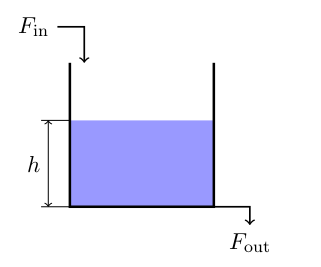
\includegraphics[width=0.5\textwidth]{tanque.png}}
   \caption{Tanque de nível}
\end{figure}

Os dados do processo são:

\begin{itemize}
\item $Q_e $ --  vazão de entrada;
\item $Q_s$  -- vazão de saída;
\item $H$    -- nível de fluído do tanque;
\item $\rho$ -- massa específico do fluído no tanque;
\item $A$    -- Área da base do tanque;
\end{itemize}

\begin{align*}
m = & \rho A H \\
m = & \frac{\partial P}{\partial t} A H + \rho \frac{\partial A}{\partial t} H + \rho A \frac{\partial H}{\partial t}
\end{align*}

Hipóteses do modelo:

Considera-se $\rho$ constante e $A$ constante, logo:

\begin{align*}
\frac{\partial m}{\partial t} = \rho A \frac{\partial H}{\partial t}
\end{align*}

Balanço de massa:

\begin{align*}
\frac{\partial m}{\partial t} = Pe Q_e - Ps Q_s
\end{align*}

Equação do sistema:

\begin{align*}
\rho A \frac{\partial H}{\partial t} = P_e Q_e - P_s Q_s \\
\frac{\partial H}{\partial t} = \frac{P_e Q_e - P_s Q_s}{\rho A}
\end{align*}

Análise Qualitativa:

\begin{itemize}
\item Se $P_s Q_s > P_e Q_e$, logo $\frac{\partial H}{\partial t} < 0 \rightarrow $  tanque esvaziando, portanto $H$ decresce;
\item Se $P_s Q_s < P_e Q_e$, logo $\frac{\partial H}{\partial t} > 0 \rightarrow $  tanque enchendo, portanto $H$ cresce;
\item Se $P_s Q_s = P_e Q_e$, logo $\frac{\partial H}{\partial t} = 0 \rightarrow $  tanque permanece igual, portanto $H$ conserva-se;
\end{itemize}

Busca-se computar o nível de fluído no tanque em função da quantidade de massa que sai do tanque. Logo, integra-se a seguinte equação:


\begin{align*}
\frac{\partial H}{\partial t} = \frac{\rho Q_e - \rho Q_s}{\rho A}
\end{align*}

Para este fim, foi escrito o seguinte programa que resolve o problema:
\pythonexternal{tanque.py}

Tendo como entrada os parâmetros abaixo:

\begin{itemize}
\item Área do tanque: $10 \phantom{0} m^2$;
\item Altura inicial de fluido no tanque: $100.0 \phantom{0} m$;
\item Intervalo de integração: $[0.0, 10.0]$;
\item Fator de discretização: $1000$;
\item Vazão de entrada: $f_{Qe}(t) = 10t  \phantom{0} l$;
\item Vazão de saída: $f_{Qs}(t) = 50 \pi cos(t)  \phantom{0} l$;
\end{itemize}

obteve-se o seguinte comportamento do sistema:

\begin{figure}[H]
\label{figure:tanque_saida}
   \center{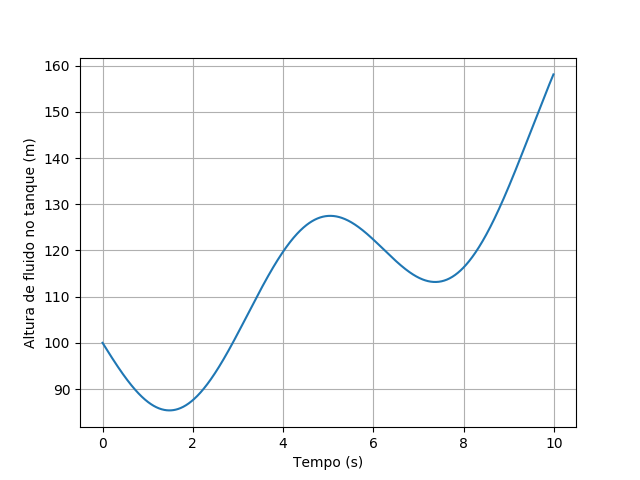
\includegraphics[width=0.5\textwidth]{saida_tanque.png}}
   \caption{Estado da altura de fluido no tanque a cada passo de tempo}
\end{figure}
\newpage
\section{Modelagem de uma viga}
Foi realizada a modelagem da vibração de uma viga Euler-Bernoulli com duas áreas seccionais distintas, esta recebendo uma frequência de vibração $\omega$, como segue abaixo:
\begin{figure}[H]
\label{figure:viga}
   \center{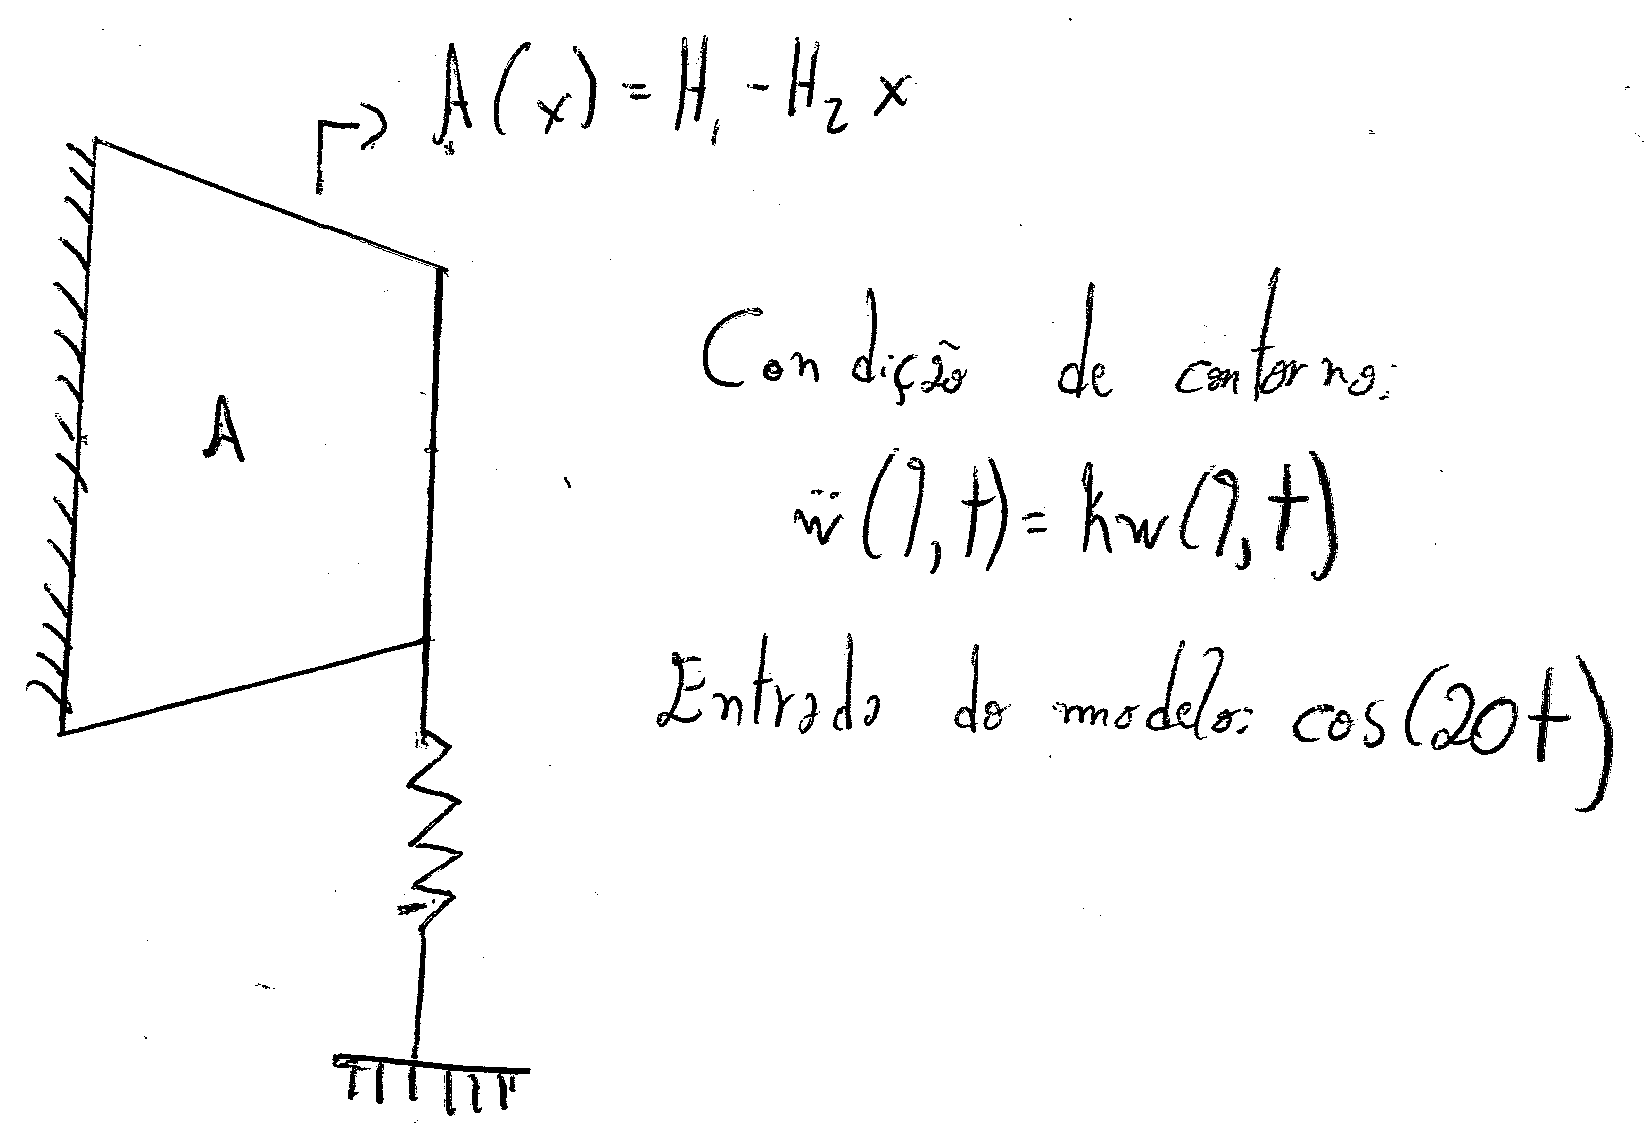
\includegraphics[width=0.75\textwidth]{viga.png}}
   \caption{Problema da viga}
\end{figure}
O sistema foi modelado a partir do método direto da rigidez, para tanto, foram obtida as matrizes de rigidez, massa e inércia, são estas:


\begin{align*}
w_{xx_{1}} = \begin{bmatrix}
96x^3 - 72x & 192x^4 - 192x^2 + 24 \\ 
192x(4x^3 - 3x) & 192x(8x^4-8x^2+1)
\end{bmatrix} 
\end{align*}

\begin{align*}
w_{xx_{2}} = \begin{bmatrix}
24x(12x^2-3) & 24x(32x^3 - 16x) \\
(12x^2-3)*(96x^2-16) & (96x^2-16)*(32x^3-16x)
\end{bmatrix} \\
\end{align*}

\begin{align*}
w_{xx_{3}} = \begin{bmatrix}
192x^3 & 576x^4 - 192x^2 \\
576x^4 - 192x^2 & \frac{9216x^5}{5} - 1024x^3 + 256x
\end{bmatrix}
\end{align*}


A análise da dinâmica do sistema se deu pela resolução da seguinte equação através do método de Euler:
\begin{align*}
R_1 u + R_2 \ddot{u} & = \vec{F} \text{\phantom{0} tal que:} \\
R_1 & = P_4 + P_1 \\
R_2 & = P_2 + P_3 \text{\phantom{0} onde:} \\
P_1 & = (w_{xx_{1}} - w_{xx_{3}})\bigm|_{x=l} - (w_{xx_{1}} - w_{xx_{3}})\bigm|_{x=0} \\
P_2 & =  \frac{-1}{k} w_{xx_{2}}\bigm|_{x=l} - w_{xx_{2}}\bigm|_{x=0}\\
P_3 & = \rho \int_{0}^{l} \begin{bmatrix}
{T_3}^2 & T_3 T_4 \\
T_4 T_3 & {T_4}^2
\end{bmatrix}
 \delta_1 - \delta_2 x\\
P_4 & = - \bigg ( cos(20t) 
\begin{bmatrix}
{T_3}^2 & T_3 T_4 \\
T_4 T_3 & {T_4}^2
\end{bmatrix} \bigm|_{x=l} \bigg ) - \bigg( cos(20t)
\begin{bmatrix}
{T_3}^2 & T_3 T_4 \\
T_4 T_3 & {T_4}^2
\end{bmatrix} \bigm|_{x=0}
\bigg ) \\
F & = \int_{0}^{1} 
\begin{bmatrix}
x cos(t) T_3 \\
x cost(t) T_4
\end{bmatrix}
\end{align*}

onde $k$ foi definido arbitrariamente como $10^6$ (constante elástica). Tais termos foram obtidos através da integração por partes do funcional de energia abaixo:
\begin{align*}
EI (H(i,x)_{xxx} H(j,x) u(i,t) \bigm|_{0}^{1} - H(i,x)_{xx} H(j,x)_{xx} H(j,x) u(i,t) \bigm|_{0}^{1} + \\
\int_{0}^{l} A(i,x)_{xx} H(j,x) u(i,t) dx) + \\
\rho A \int_{0}^{1} H(i,x) H(j,x) \ddot{u} (i,t) dx = \int_{0}^{1} f(x,t) H(j,x) dx 
\end{align*}
onde $A = H_1 - H_2x$

Após isso, um experimento foi criado a fim de observar a frequência de vibração da viga dado um sinal de entrada da forma $cos(\omega t)$. O experimento teve os seguintes parâmetros:
\begin{itemize}
\item Constante Elástica $k$: $10^{6}$
\item $\rho$: $3.0$;
\item Largura inicial da viga: $0.9$ m;
\item Largura final da viga: $0.1$ m;
\item Funções de Forma: Polinômios de Hermite $T_3$ e $T_4$ $\rightarrow$ $4x^3-3x$ e $8x^4-8x^2+1$;
\item Frequência de vibração na barra: $\omega = cos(20t)$;
\item Tempo simulado: $10 \phantom{0} s$
\item Fator de discretização: $10000$
\item Comprimento da viga: $15 \phantom{0} m$
\end{itemize}

\begin{figure}[H]
\label{figure:tanque}
   \center{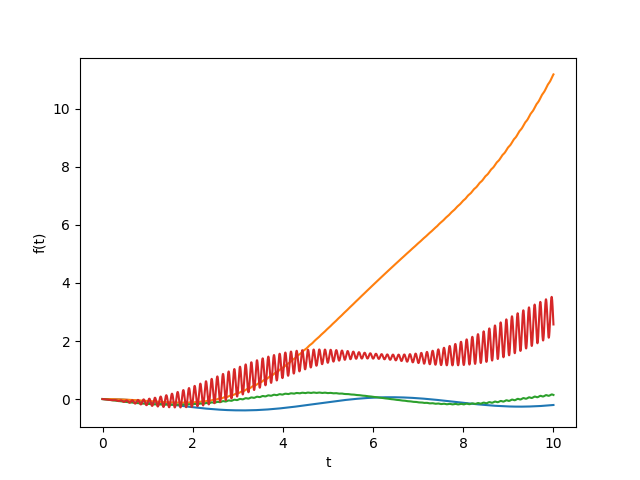
\includegraphics[width=0.8\textwidth]{saida_viga.png}}
   \caption{Simulação da dinâmica da viga em função do tempo \\
            Em vermelho e azul respectivamente: Deslocamento vertical e derivada \\
            Em verde e laranja respectivamente: Deslocamento horizontal e derivada}
\end{figure}

Notou-se que (independente da frequência de entrada) vigas com grandes diferenças entre larguras finais e iniciais possuem uma frequência de vibração mais elevada, necessitando de um fator de discretização maior no método de Euler, a fim de que a dinâmica da mesma seja simulada corretamente.

A implementação abaixo reproduz o experimento descrito:
\pythonexternal{viga.py}

\newpage

\section{Modelagem de um Flip-Flop RS}
Foi realizada a modelagem do Flip-Flop RS abaixo:

\begin{figure}[H]
\label{figure:flipflop}
   \center{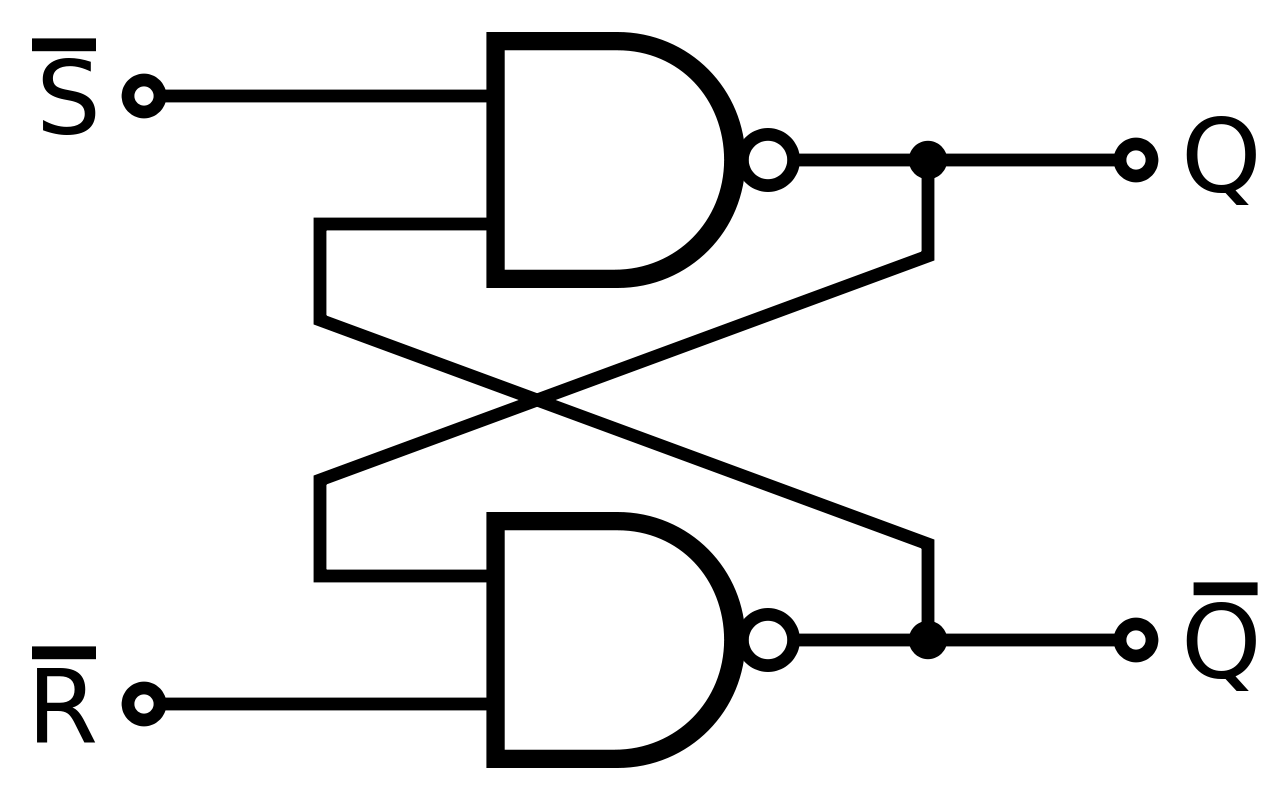
\includegraphics[width=0.33\textwidth]{ffrs.png}}
   \caption{Flip Flop RS Síncrono}
\end{figure}


A saída do Flip-Flop RS no instante $k+1$ é dada pelas equações abaixo:
\begin{align*}
f(x_1,x_2,x_3) = \overline{x_3^{(k+1)}} = \overline{\bigg (x_1^{(k)}+\overline{\bigg (x_2^{(k)}+\overline{x_3^{(k)}} \bigg )} \bigg )} \\
f(x_1,x_2,x_3) = x_3^{(k+1)} = \overline{\bigg (x_2^{(k)}+ \overline{\bigg (x_1^{(k)}+x_3^{(k)} \bigg )} \bigg )}
\end{align*}


Logo, têm-se a seguinte tabela verdade:
\begin{longtable}[c]{|l|l|l|l|}
\hline
$S$ & $R$ & $Q_{ant}$ & Saída \\ \hline
\endfirsthead
%
\multicolumn{4}{c}%
{{\bfseries Table \thetable\ continued from previous page}} \\
\hline
$S$ & $R$ & $Q_{ant}$ & Saída \\ \hline
\endhead
%
0 & 0 & 0    & 0     \\ \hline
0 & 0 & 1    & 1     \\ \hline
0 & 1 & 0    & 0     \\ \hline
0 & 1 & 1    & 0     \\ \hline
1 & 0 & 0    & 1     \\ \hline
1 & 0 & 1    & 1     \\ \hline
1 & 1 & 0    &  (Estado não permitido)    \\ \hline
1 & 1 & 1    &  (Estado não permitido)     \\ \hline
\caption{Tabela Verdade do Flip Flop RS}
\label{tab:FFRS_TabelaVerdade}\\
\end{longtable}


O gráfico abaixo demonstra o comportamento do Flip-Flop RS sob a seguinte entrada:


\begin{itemize}
\item Comprimento do sinal: 1024 bits;
\item Sinal da entrada de $R$: $5 \pi t$;
\item Sinal da entrada de $S$: $10 \pi t$;
\item Sinal da entrada de $Q_{ant}$: $15 \pi t$;
\end{itemize}

\begin{figure}[H]
\label{figure:ffrs}
   \center{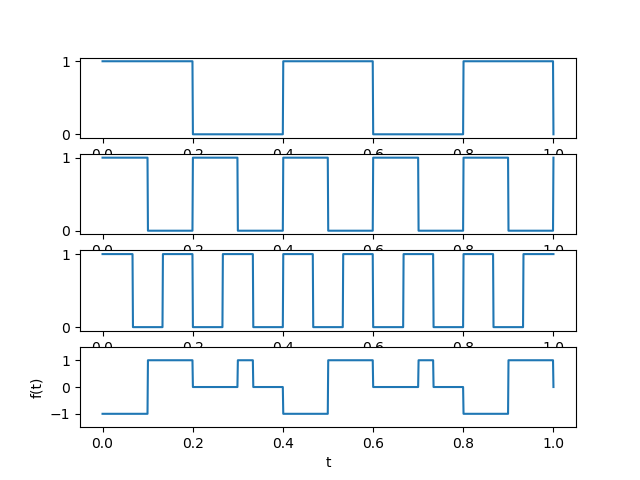
\includegraphics[width=0.75\textwidth]{ffrs_saida.png}}
   \caption{Simulação do Flip-Flop RS - Considere -1 como estado proibido}
\end{figure}
O experimento pode ser replicado através do código abaixo:

\pythonexternal{ffrs.py}


\newpage

%\section{Modelagem de um Circuito de 2ª Ordem}
%\newpage

\section{Modelagem de um Filtro Gaussiano}
O filtro gaussiano será modelado a partir do seguinte filtro passa-baixo:

\begin{figure}[H]
\label{figure:pulsoGaussiano}
   \center{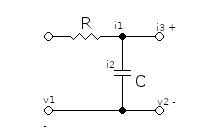
\includegraphics[width=0.3\textwidth]{filtroPassaBaixo.png}}
   \caption{Filtro passa-baixo genérico}
\end{figure}
Temos que:

\begin{align*} 
i_1 & = i_2 + i_3 \\
i_3 & = i_1 - i_2
\end{align*}  

\begin{align*}
\frac{v_3}{R} & = \frac{v_1}{R} - C\dot v_2 \\
v_3 & = v_1 - RC \dot v_2 \text{ visto que } v_2 = v_3 \\
\frac{\dot v_2}{R} & = \frac{v_1}{R} - C \dot v_2 \\
v_2 & = v_1 - Rc \dot v_2 \hfill
\end{align*}
Aplica-se Transformada de Laplace para ir do domínio do tempo para domínio da frequência
\begin{align*}
v_2 & = v_1 - RCSv_2 (S \in \mathbb{C} \text{ é o domínio da função)} \\
v_1 &  = v_2 \cdot (1+RCS) \cdot v_2
\end{align*}


Relação de entrada/saída:
\begin{align*}
T & = \frac{\text{Saída}}{\text{Entrada}} \\
T & = \frac{v_2}{v_1} = \frac{1}{1+RCS} \phantom{0}\bigg ( S = S_1+j_1 \bigg ) \phantom{000} \text{Função de Transferência} \\
T & = c{v_2}{v_1} = \frac{1}{(1+RCS_1) + jRC_\omega} \cdot \frac{(1+RCS_1)-jRC \omega}{(1+RCS)-jRC \omega} = \frac{1+RCS_1-jRC \omega}{(1+RCS_1)^2+(R C \omega)^2}
\end{align*}

Estabilidade no domínio da frequência ($Re(T)$ denota a parte real de $T$):
\begin{align*}
Re(T) \leq 0 && 1+RCS_1<0 = S_1 L - \frac{1}{RC}
\end{align*}
\begin{align*}
\frac{1}{RC} & = \text{constante de tempo}
\end{align*}
Se $Re(T)>0$, então sistema é instável:\newline
Supondo que $S_1 = 0$, temos que:

\begin{align*}
T & = \frac{1}{1+jRC \omega} \cdot \frac{1-jRC \omega}{1-jRC \omega} = \frac{1-jRC \omega}{1-(RC \omega)^2} \\
T & = \frac{1}{1+(RC\omega)} - j \frac{RC \omega}{1+(Rc\omega)^2} \\
|T|^2 & = \frac{1}{(1+(RC \omega)^2)^2} + \frac{(RC \omega)^2}{(1+(RC \omega)^2)^2} = \frac{1+(RC \omega)^2}{(1+(RC \omega)^2)^2} = \frac{1}{1+(RC \omega)^2} \\
|T| & = \frac{1}{(1+(RC \omega)^2)^{0.5}}
\end{align*}


\begin{align*}
arg(T) & = \frac{\frac{RC \omega}{1+(RC \omega)^2}}{\frac{1}{1+(RC \omega)^2}} = \frac{-RC \omega}{1+(RC \omega)^2} \cdot (1+(RC \omega)^2) = \\
arg(T) & = \tan^{-1} v_1 = \tan^{-1} (RC \omega) = \theta
\end{align*}

\begin{align*}
l & = \bigg ( \frac{1}{(1+R^2 C^2 \omega^2)^{0.5}} \bigg ) \\
T & = l \cdot (\cos(-\tan^{-1}(R C \omega))+ j \sin (-tan^{-1} (R C \omega)) ) \\
T & = e^{(1+ R^2 C^2 \omega^2)^{-0.5}} \cdot (\cos \theta - j \sin \theta) \\
\end{align*}

\begin{align*}
\frac{1}{(1+R^2 C^2 \omega^2)^{0.5}} & \rightarrow \text{Constante de Tempo}
\end{align*}

A implementação em Python abaixo gera um pulso de sinal modelado através das equações desenvolvidas anteriormente:

\pythonexternal{pulsoGaussiano.py}

O gráfico abaixo foi gerado através do código com os seguintes parâmetros de entrada:

\begin{itemize}
\item Largura de banda no domínio da frequência: 0.5 Hz;
\item Nível de referência no qual a largura de banda é calculada: -6.0 dB;
\item Limiar de truncamento: -60.0 dB
\end{itemize}

\begin{figure}[H]
\label{figure:pulsoGaussiano}
   \center{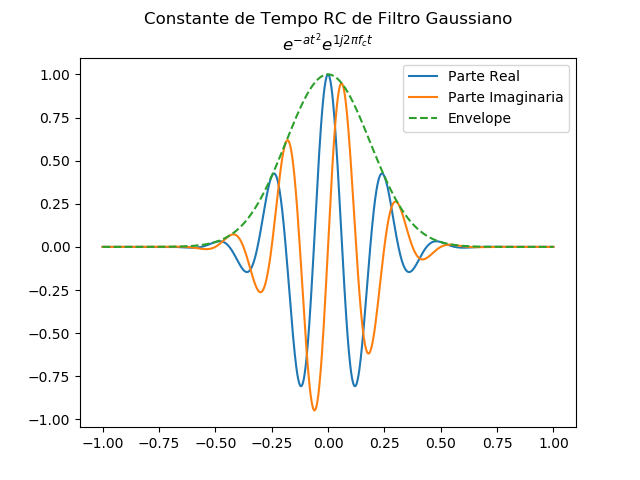
\includegraphics[width=0.5\textwidth]{pulsoGaussiano.png}}
   \caption{Pulso Gaussiano gerado pela execução do código}
\end{figure}

No gráfico seguinte, é apresentada a variação da saída da parte real do circuito sob diferentes frequências do filtro:

\begin{figure}[H]
\label{figure:pulsoGaussiano}
   \center{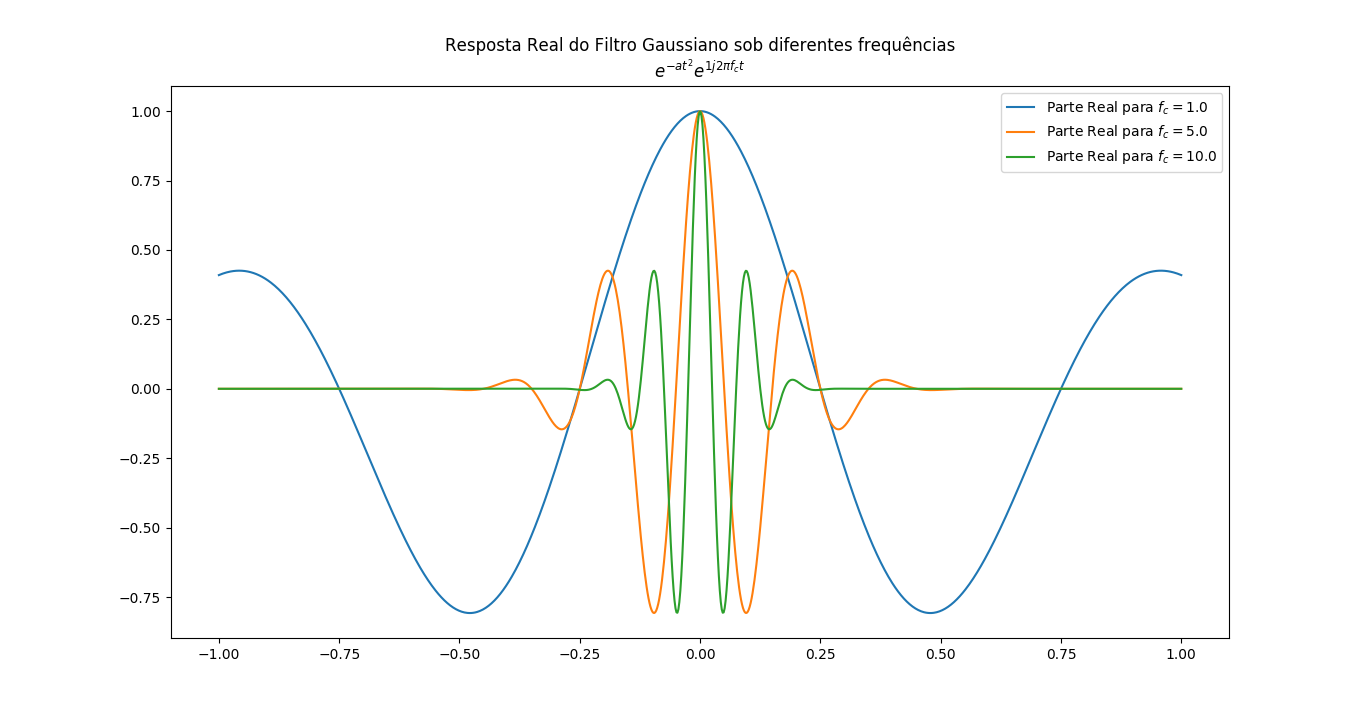
\includegraphics[width=0.5\textwidth]{pulsoGaussianoDiferentesFrequencias.png}}
   \caption{Saída Real do Filtro Gaussiano para diferentes frequências}
\end{figure}
\newpage
\section{Modelagem de um circuito RLC}
\subsection{Circuito 1}
Considerando o circuito abaixo:

\begin{figure}[H]
\label{figure:circuito_1}
   \center{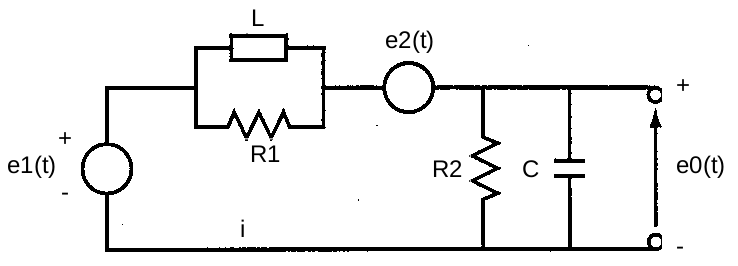
\includegraphics[width=0.5\textwidth]{circuito_1.png}}
   \caption{Circuito RLC}
\end{figure}

Foi criado um modelo do tipo $f(e_1(t),e_2(t)) = e_0(t)$ em função das correntes:

Tem-se que:

\begin{align*}
i_C + i_{R2} + i_2 = 0 \\
i_2 = i_{R1} + i_L \text{\phantom{0}logo:} \\
i_C + i_{R2} + i_{R1} + i_{L} = 0 \text{\phantom{0}(Lei de Kirchoff)}
\end{align*}

Para cada elemento do circuito, temos que:

\begin{align*}
i_{R1} = \frac{1}{R_1} (e_0 + e_2 - e_1) \\
i_{R2} = \frac{e_0}{R_2} \\
i_C = C \frac{de_0}{dt} \\
i_L = i_L(0) + \frac{1}{L} \int_{0}^{1} (e_0 + e_2 - e_1) dt
\end{align*}

Logo, a dinâmica do sistema é dada por:

\begin{align*}
e_{0}(t) = \frac{1}{R_1}  (e_1(t) - e_2(t)) + \frac{1}{L} \int_{0}^{t} (e_1(t) - e_2(t)) dt - i_{L}(0)
\end{align*}
\newpage
\subsection{Circuito 2}
Foi modelado o circuito abaixo:

\begin{figure}[H]
\label{figure:circuito_2}
   \center{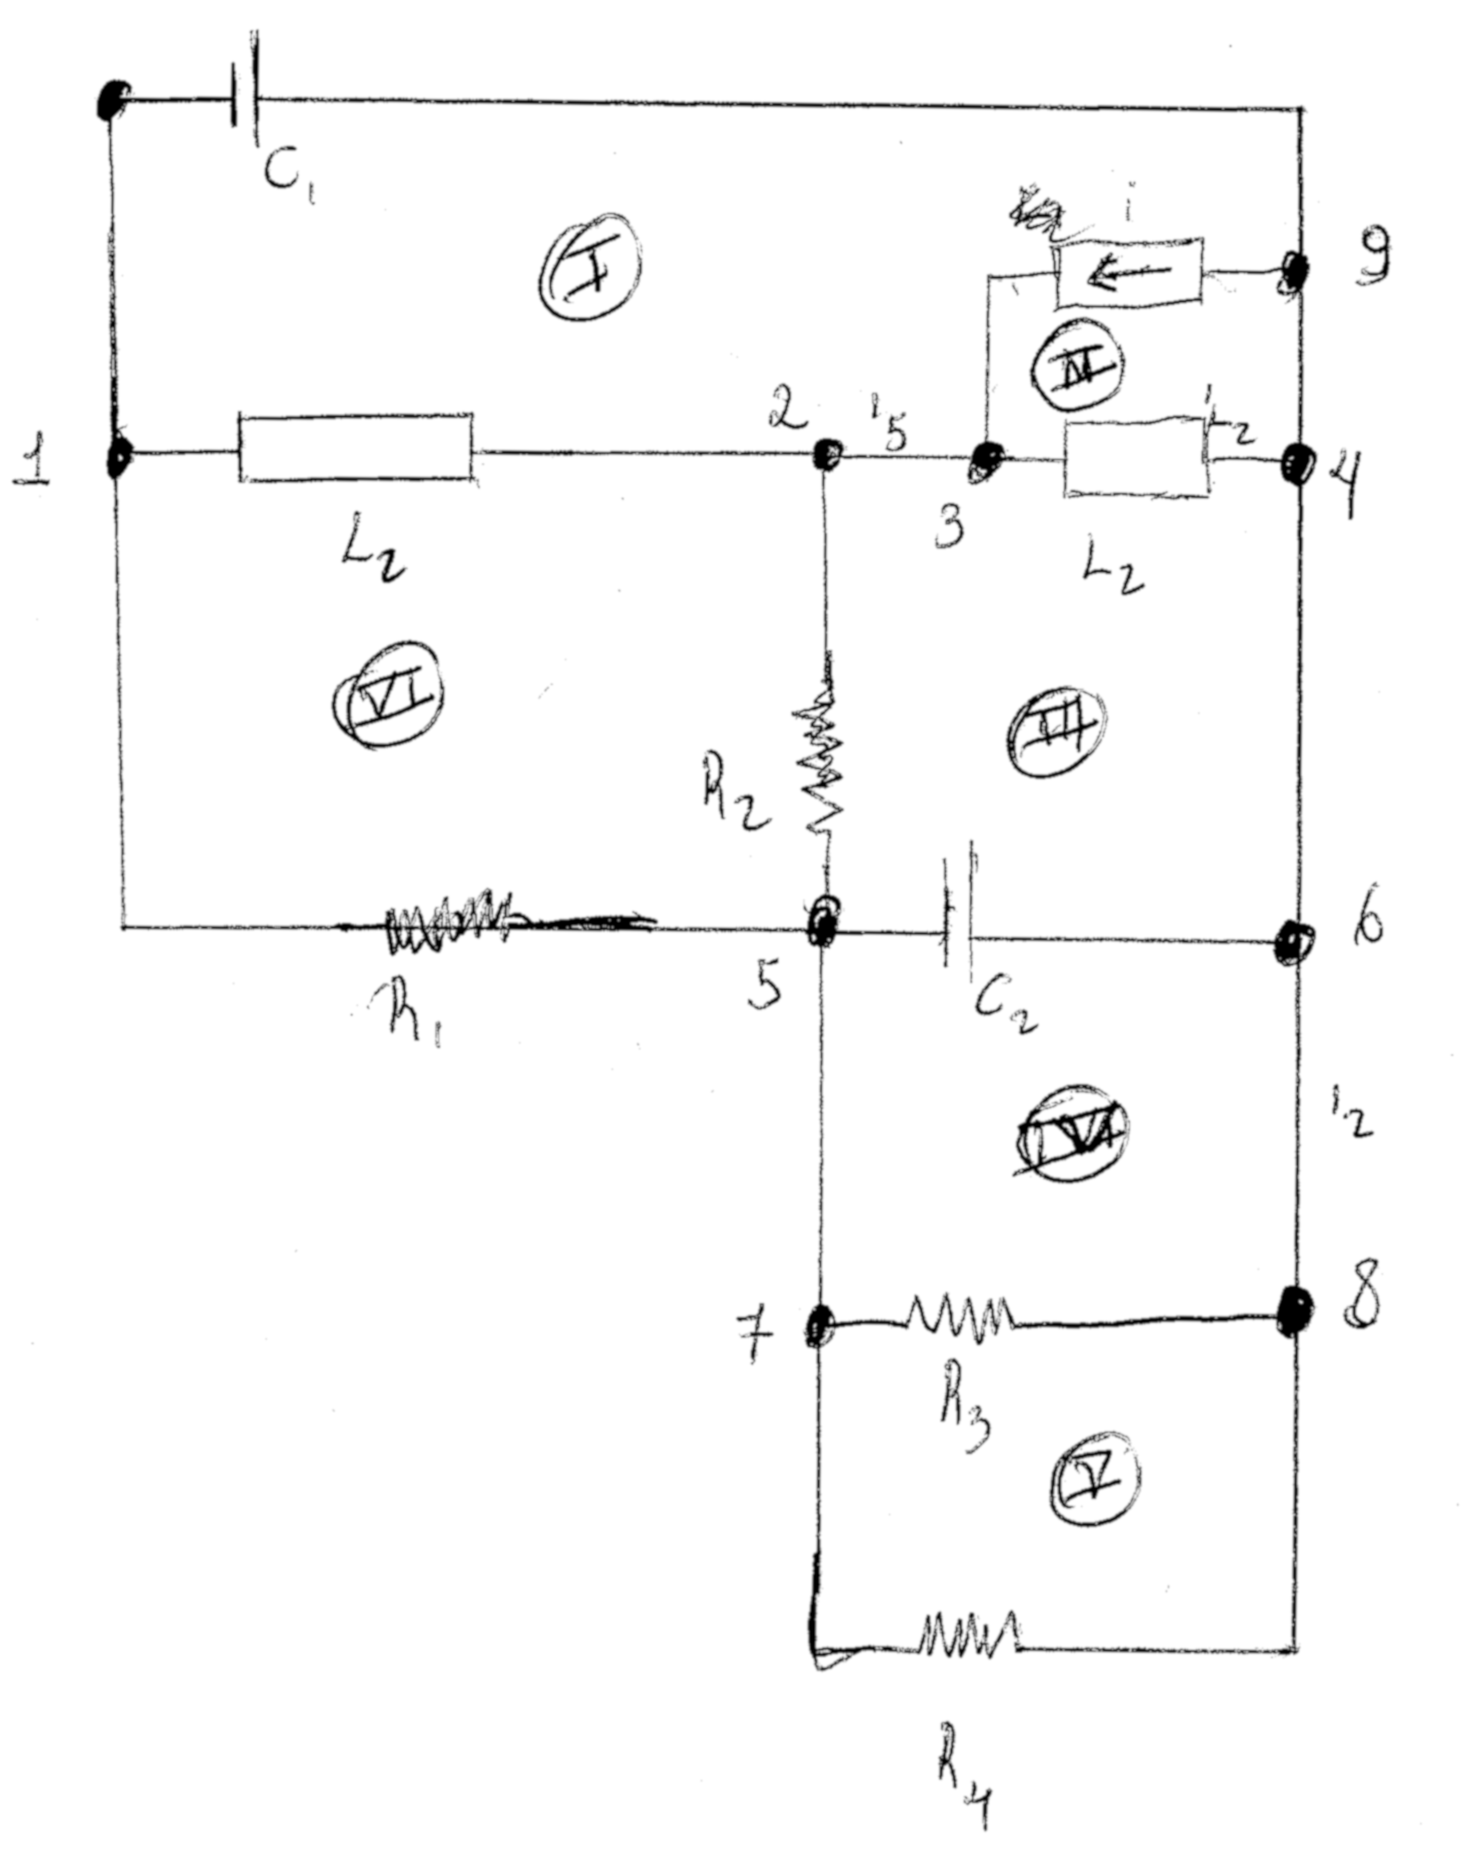
\includegraphics[width=0.5\textwidth]{circuito_2.png}}
   \caption{Circuito RLC}
\end{figure}

Pela Lei de Kirchoff temos a seguinte análise nodal:

\begin{align*}
\left\{\begin{matrix}
\text{nó 1} \rightarrow &  i_{L_{1}} + i_{L_2} + i_{R_1} & = 0 \\
\text{nó 2} \rightarrow &  i_{L_{1}} + i_{R_2} + i_{5} & = 0 \\
\text{nó 3} \rightarrow &  i_{5} + i + i_{L_2} & = 0 \\
\text{nó 4} \rightarrow &  i_{L_2} + i_{4} + i_3 & = 0 \\
\text{nó 5} \rightarrow &  i_{R_1} + i_{R_2} + i_{L_2} + i_1 & = 0 \\
\text{nó 6} \rightarrow &  i_{L_2} + i_3 + i_2 & = 0 \\
\text{nó 7} \rightarrow &  i_1 + i_{R_4} + i_{R_3} & = 0 \\
\text{nó 8} \rightarrow &  i_{R_4} + i_{R_3} + i_{2} & = 0 \\
\text{nó 9} \rightarrow &  i_{L_1} + i + i_{1} & = 0 
\end{matrix}\right.
\end{align*}

Também pela Lei de Kirchoff, as tensões são expressas da seguinte forma:
\begin{align*}
\left\{\begin{matrix}
V_{C_1} - V_{i} + V_{L_{1}} & = 0 \\
V_{i} + V_{L_{2}} & = 0 \\
V_{L_{2}} + V_{R_{2}} + V_{C_{2}} & = 0 \\
V_{L_2} + V_{R_3} & = 0 \\
V_{R_3} + V_{R_4} & = 0 \\
V_{L_1} + V_{R_2} + V_{R_1} & = 0
\end{matrix}\right.
\end{align*}



Uma vez que o modelo foi implementado, foram utilizados os seguintes parâmetros no experimento:

\begin{itemize}
\item $R_1: $ 1 $\Omega$;
\item $R_2: $ 2 $\Omega$;
\item $R_3: $ 3 $\Omega$;
\item $R_4: $ 4 $\Omega$;

\item $C_1: $ $1 \times 10^{-9} F$;
\item $C_2: $ $2 \times 10^{-9} F$;

\item $L_1: $ $1 \times 10^{-9} H$;
\item $L_2: $ $2 \times 10^{-9} H$;

\item Tensão da fonte: $1 \text{\phantom{0} A}$; 
\item Tempo simulado: $7 \times 10^{-5} \text{\phantom{0}} s$ (devido ao rapido equilíbrio do sistema)
\end{itemize}

Foram obtidos os seguintes resultados:

\begin{figure}[H]
\label{figure:circuito_2}
   \center{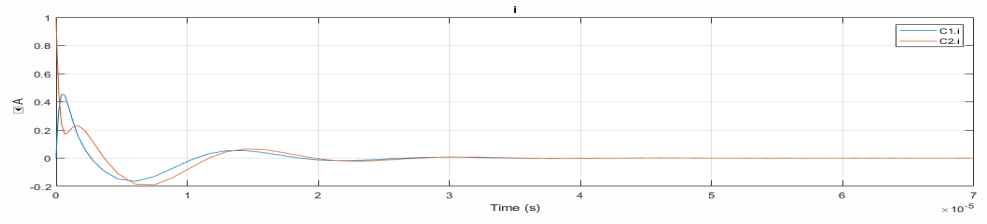
\includegraphics[width=0.9\textwidth]{c2Ca.png}}
   \caption{Corrente nos capacitores $C_1$ e $C_2$}
\end{figure}

\begin{figure}[H]
\label{figure:circuito_2}
   \center{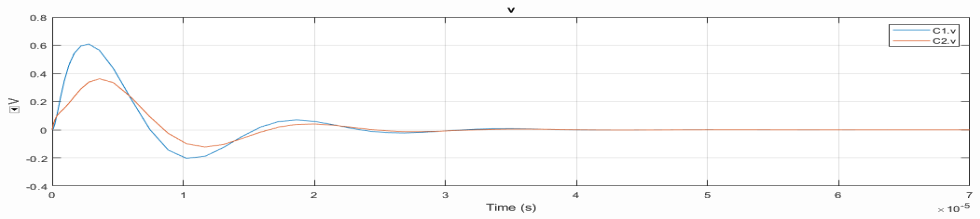
\includegraphics[width=0.9\textwidth]{c2Cv.png}}
   \caption{Tensão nos capacitores $V_1$ e $V_2$}
\end{figure}

\begin{figure}[H]
\label{figure:circuito_2}
   \center{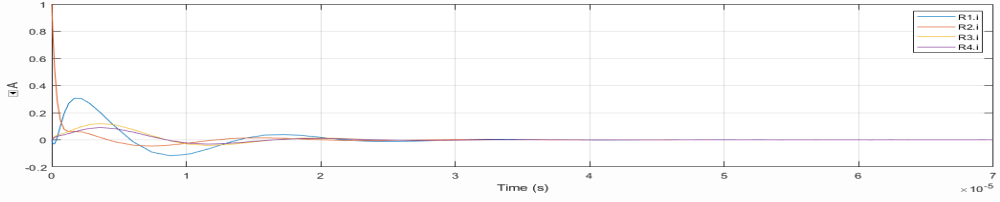
\includegraphics[width=0.9\textwidth]{c2Ra.png}}
   \caption{Corrente nas resistências $R_1$, $R_2$, $R_3$ e $R_4$}
\end{figure}

\begin{figure}[H]
\label{figure:circuito_2}
   \center{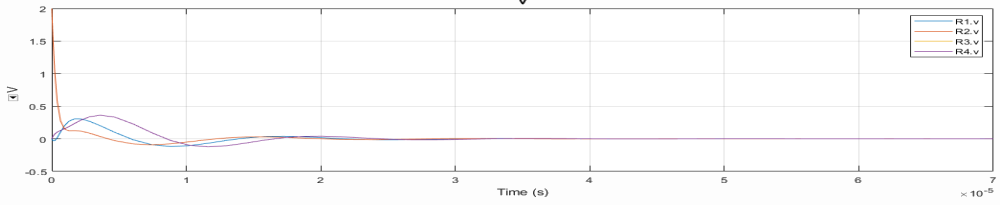
\includegraphics[width=0.9\textwidth]{c2Rv.png}}
   \caption{Tensão nas resistências $R_1$, $R_2$, $R_3$ e $R_4$}
\end{figure}

\begin{figure}[H]
\label{figure:circuito_2}
   \center{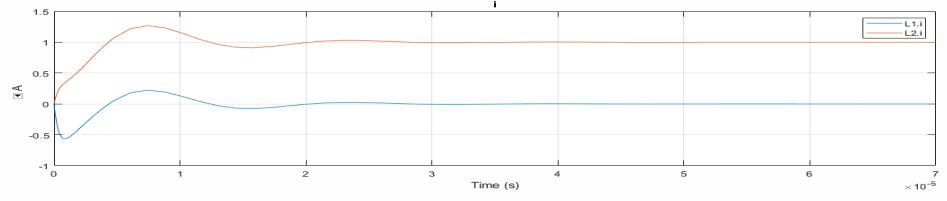
\includegraphics[width=0.9\textwidth]{c2Ia.png}}
   \caption{Corrente nos indutores $L_1$ e $L_2$}
\end{figure}

\begin{figure}[H]
\label{figure:circuito_2}
   \center{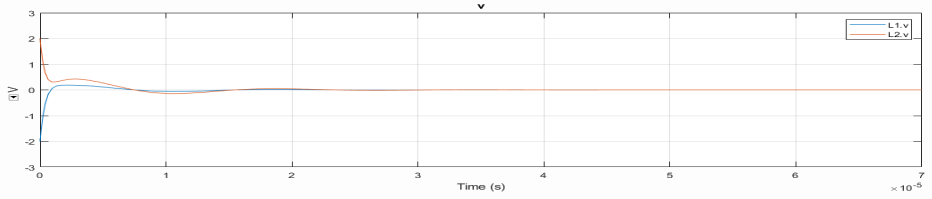
\includegraphics[width=0.9\textwidth]{c2Iv.png}}
   \caption{Tensão nos indutores $L_1$ e $L_2$}
   \end{figure}

\begin{figure}[H]
\label{figure:circuito_2}
   \center{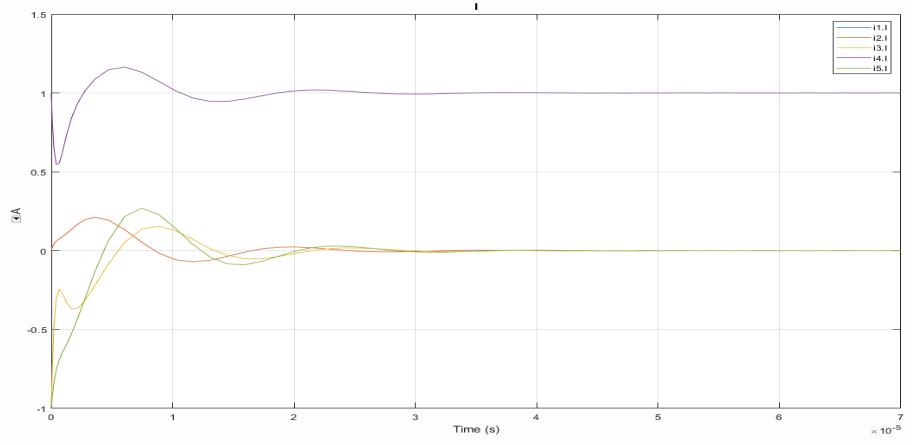
\includegraphics[width=0.9\textwidth]{c2i.png}}
   \caption{Correntes $i_1$, $i_2$, $i_3$, $i_4$ e $i_5$}
   \end{figure}

\newpage
\section{Modelagem de um motor de corrente contínua}
Foi realizada a modelagem do motor DC abaixo, a fim de simular a corrente elétrica e velocidade no motor:
\begin{figure}[H]
\label{figure:circuito_2}
   \center{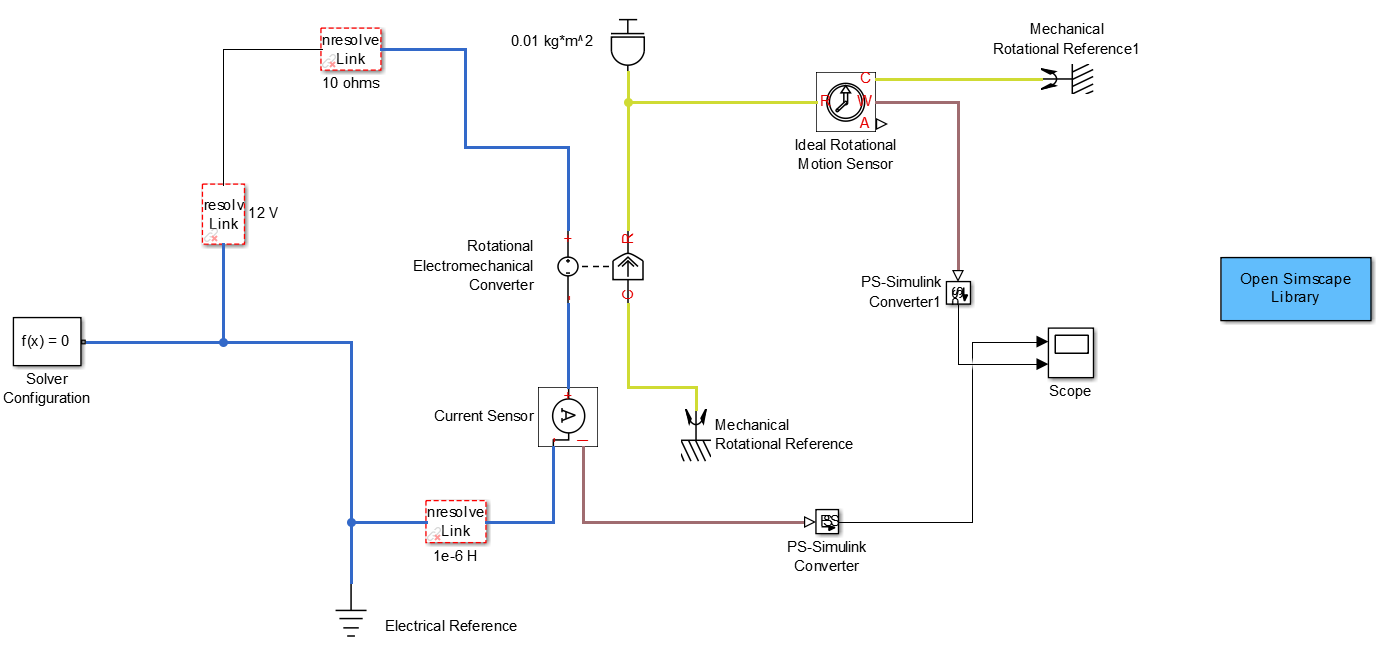
\includegraphics[width=0.9\textwidth]{motor_dc.png}}
   \caption{Circuito RLC}
\end{figure}
Para tanto, foi integrado o seguinte sistema de equações diferenciais ordinárias:

\begin{align*}
\left\{\begin{matrix}
L \frac{di}{dt} + Ri + K & = V \\
I \frac{d \omega}{dt} &= Ki
\end{matrix}\right.
\end{align*}
Foram utilizados os seguintes parâmetros no experimento:


\begin{itemize}
\item Resistência: $\phantom{0} 10 \Omega$;
\item Tensão da fonte: $\phantom{0} 12 V$;
\item Indutânica: $\phantom{0} 1 mH$ (milihenrie);
\item Inércia do sistema: $\phantom{0} 10^{-2}\phantom{0} kg m^2$
\item Razão Tensão/Frequência do motor: 0.1 $\phantom{0} V/rad/s$

Obteve-se a seguinte saída:

\begin{figure}[H]
\label{figure:circuito_2}
   \center{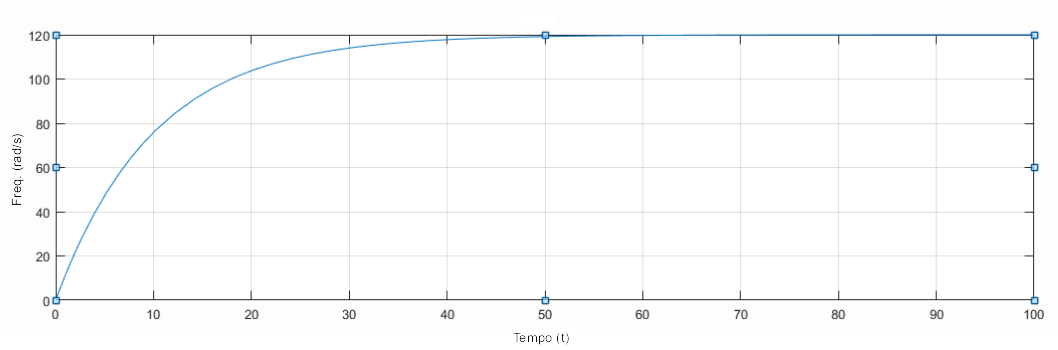
\includegraphics[width=0.9\textwidth]{frequencia_motor.png}}
   \caption{Frequência do motor DC no experimento}
\end{figure}

\begin{figure}[H]
\label{figure:circuito_2}
   \center{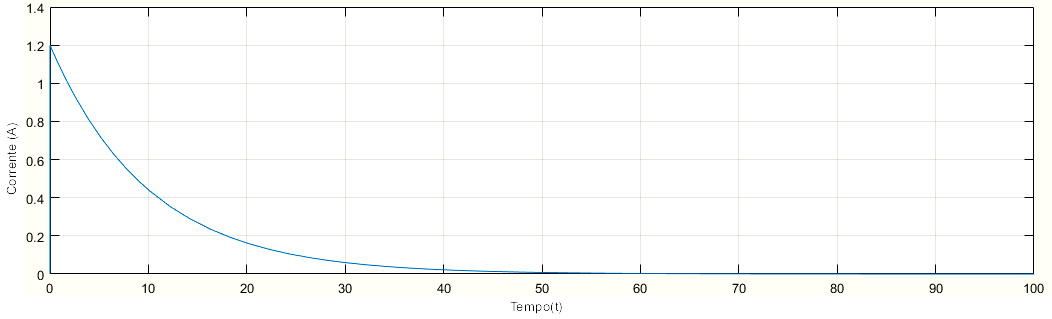
\includegraphics[width=0.9\textwidth]{corrente_motor.png}}
   \caption{Corrente elétrica através motor DC no experimento}
\end{figure}

\end{itemize}
\end{document}